\chapter{Models}
Let's begin the chapter with a question. Why do we need models?
Well, they represent a good approximation of the real world and allow describing events through a parametric representation (parameters can be extracted and used for processing). In the context of computer vision, models are used to describe the geometry of the world, the appearance of objects, and the imaging process. In this chapter, we will discuss the most common models used in computer vision. We will start with the pinhole camera model,then we will see the perspective projection model and finally, we will discuss the appearance model.
\section{The Pinhole Camera Model}
The pinhole camera model is the simplest model used to describe the imaging process. It is based on the principle that light travels in straight lines. The model is composed of a pinhole, a plane, and an image plane. The pinhole is a small hole in the plane, and the image plane is placed behind the pinhole. The light rays coming from the scene pass through the pinhole and project the scene onto the image plane. 
\begin{figure}[h]
    \centering
    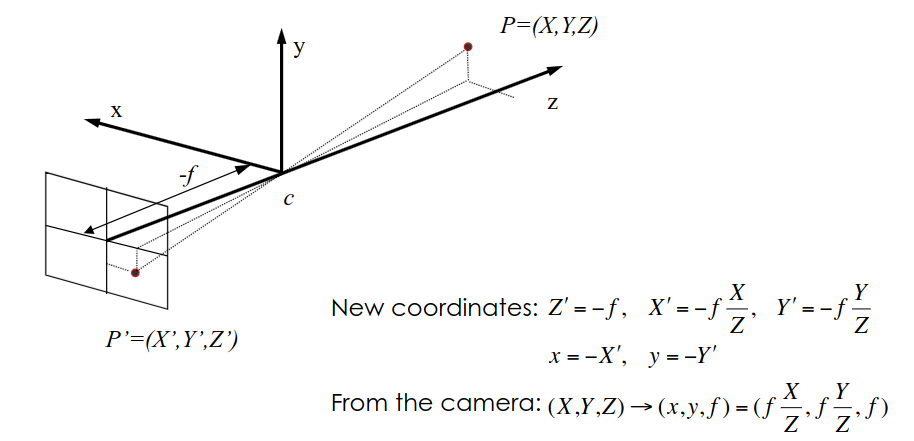
\includegraphics[width=1\textwidth]{Figures/Pinhole.png}
\end{figure}
\\\textit{PS: If the object is far, it appears small in the image. If the object is close, it appears large in the image.}
\subsection{Features of the Pinhole Camera Model}

\begin{figure}[H]
    \centering
    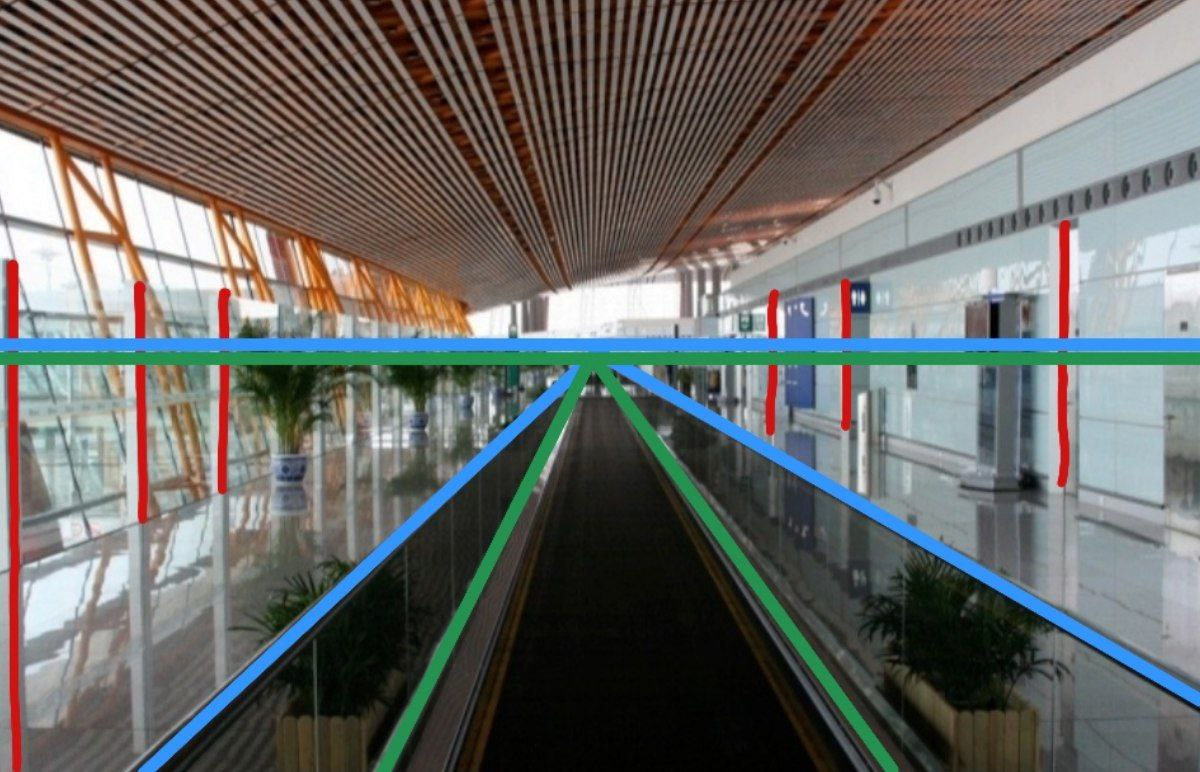
\includegraphics[width=0.5\textwidth]{Figures/horizon.jpg}
    \caption{The behavior lines in the world and in the image.}
    \label{fig:horizon}
\end{figure}
\begin{itemize}
    \item Parallel lines in the world converge to a single point in the image;
    \item Parallel lines on the same plane lead to \textit{collinear vanishing} points. In Figure \ref{fig:horizon} we can see how the blue and green lines that lie parallel on two different planes, eveltually converge to the same point in the image plane;
    \item The line where coplanar parallel lines end up is called the \textit{horizon} for that plane;
    \item Vertical lines (red) are perpendicular to the horizon.
\end{itemize}

\begin{figure}[H]
    \centering
    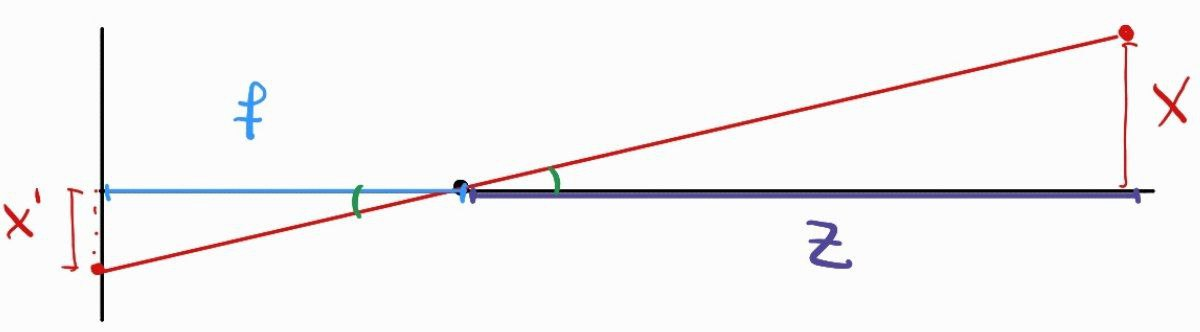
\includegraphics[width=0.5\textwidth]{Figures/triangles.jpg}
    \caption{Similar triangles in the projection.}
    \label{fig:triangles}
\end{figure}

The intuition behind the projection of the pinhole camera model is based on the concept of similar triangles. In Figure \ref{fig:triangles} we can see how the triangles formed by the object and the image plane are similar, \(f\) is the \textit{focal length} of the camera, \(Z\) is the distance of the object to the pinhole and \(X\) and \(X'\) are respectively the position of the object and its projection on the image plane. This means that the ratio of the sides of the triangles is the same, this concept is used to derive the projection equations. 


\section{Projection}
The projection is the process of mapping 3D points (+time) to 2D points. The projection of a 3D point onto the image plane is defined by a line that passes through the point and the center of projection. The intersection of this line with the image plane gives the 2D projection of the 3D point. 
\[
    f: \mathbb{R}^4 \rightarrow \mathbb{R}^3    
\]
\[
    f(X,Y,Z,t) = (x,y,t)
\]
\textit{NB: contiuous variables.}       
\\
Exist two types of projection:
\begin{itemize}
    \item Perspective projection;
    \item Orthographic projection.
\end{itemize}
\subsection{The Perspective Projection Model}
The perspective projection model is an extension of the pinhole camera model. It is used to describe the imaging process in a more realistic way. The model is based on the principle that light travels in straight lines and that the image is formed by the intersection of these lines with the image plane. 
For simplicity we usually consider the image plane on the same side of the “real world”, to avoid the picture flip.
\begin{figure}[h]
    \begin{subfigure}{0.5\textwidth}
        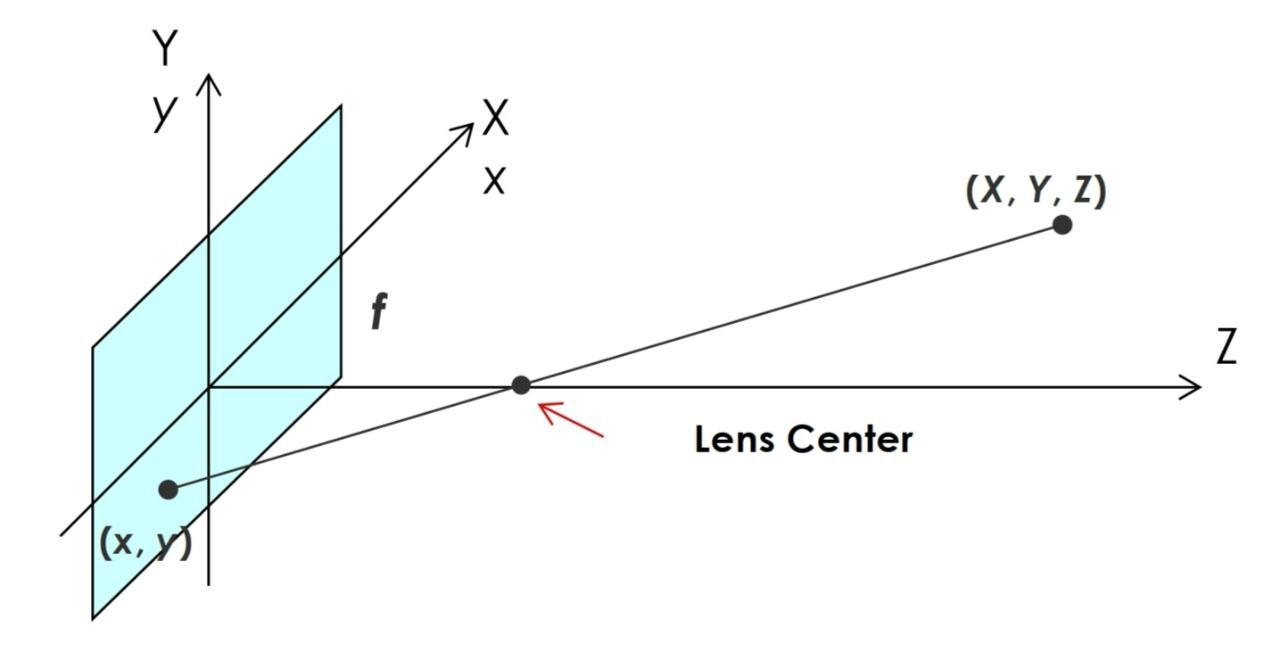
\includegraphics[scale=0.2]{Figures/Perspective_proj1.jpeg} 
        \label{fig:subim1}
    \end{subfigure}
    \begin{subfigure}{0.5\textwidth}
        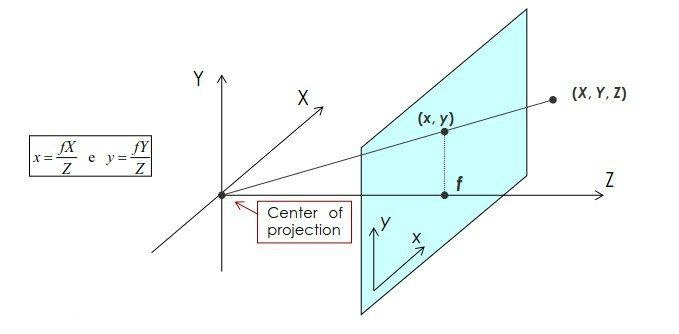
\includegraphics[scale=0.4]{Figures/Perspective_proj.jpeg}
        \label{fig:subim2}
    \end{subfigure}
        \label{fig:image2}
\end{figure}
The center of projection corresponds to the origin of the 3D space. The plane (X,Y) is parallel to (x,y). 
\\\textit{PS: This approximation is allowed when Z$>>$f.}
\\From a computational point of view nothing changes, we simply shift the image plane from back to front in order to have the image straight. For what concerns the projection, we can use the same formulas as before but we remove the minus f from the denominator(too small).
\[
    \begin{cases}
        \frac{x}{f} = \frac{X}{Z-f} \\
        \frac{y}{f} = \frac{Y}{Z-f}
    \end{cases} \Rightarrow \begin{cases}
        x = \frac{fX}{Z-f} \\
        y = \frac{fY}{Z-f}
    \end{cases} \Rightarrow \begin{cases}
        x = \frac{fX}{Z} \\
        y = \frac{fY}{Z}
    \end{cases}
\]

\subsection{The Orthographic Projection Model}
The orthographic projection model is a simplified version of the perspective projection model. It is assumed that all rays originated from the 3D object, and from the scene in general, are parallel among each other. 
In the drawing, the image plane is parallel to (X,Y).
\begin{figure}[h]
    \centering
    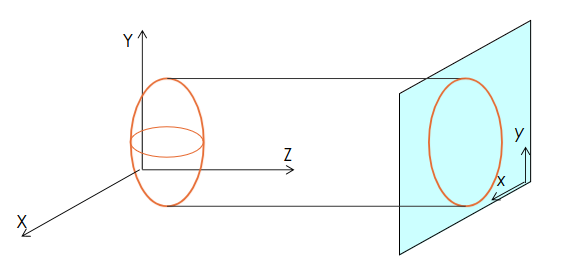
\includegraphics[width=0.5\textwidth]{Figures/Orthographic_proj.png}
\end{figure}
\\Assuming that the image plane is parallel to (X,Y), the orthographic projection
can be simply described in Cartesian coordinates as:
\[
    \begin{cases}
        x = X \\
        y = Y
    \end{cases}
\]
Or in form of a matrix:
\[
    \begin{bmatrix}
        x \\
        y
    \end{bmatrix} = \begin{bmatrix}
        1 & 0 & 0 \\
        0 & 1 & 0
    \end{bmatrix} \begin{bmatrix}
        X \\
        Y \\
        Z
    \end{bmatrix}   
\]
\textit{NB: The distance of the object from the camera does not affect the intensity of the image projected onto the 2D plane.
It is a good approximation when the distance of the object is much bigger than the depth of the object itself. }

\section{Illumination Models}
Illumination is a key element, it models the appearance/perception of objects.
When a light source hits an object, light can be absorbed, reflected, or transmitted.
It’s very complex to model, we perceive objects because they reflect light in specific wavelengths. Reflection can be specular or diffuse.
Specular means that more energy is concentrated in the light source direction.
While in diffuse the energy is constant in all directions, and the position of the observer is irrelevant.
Different surfaces vary in specularity, some of them (matte) reflect light uniformly in all directions, while glossy objects reflect light in specific directions.
It also depends on the distance and the inclination of the light source.
The problem is to determine how the surface is irradiated by the light source.We can make an assumption that the light source is far away, so we can assume that all rays can be represented by a single unit vector s (orthographic projection).
For each surface element (btw dashed lines) the light is irradiated considering the cosine of the angle between the surface normal and the light direction.
\begin{figure}[h]
    \centering
    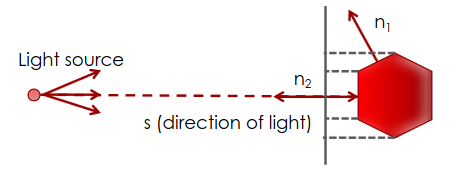
\includegraphics[width=0.5\textwidth]{Figures/Illumination.png}
\end{figure}
\\\textit{NB: intensity we perceive is equal to dot product of the normal of the surface and the light direction. Dot product $\Rightarrow$ cosine $\Rightarrow$ more close to 90 degrees, less we see.}
\subsection{Lambertian Reflectance}
Is a model for diffuse reflection, it is based on the assumption that the surface is rough enough w.r.t. the light wavelength. This means that each surface element reflects light evenly in all directions. The luminance of the surface is the same regardless of the viewing angle. The specular component is neglected.
\\\textit{Assumes that the surface we're dealing with is ideal, so looking at it from any angle we'll see the same intensity.}
\[
    I = \rho n \cdot s
\]
Where:
\begin{itemize}
    \item I is the intensity of the light;
    \item $\rho$ is the albedo, the ratio of the reflected illumination to the total illumination, intrinsic property of the surface (not true hihih, some surfaces may reflect light differently depending on the view angle);
    \item n is the normal to the surface;
    \item s is the direction of the light.
\end{itemize}
An element is not visible if the angle between the normal and the light direction is greater than 90 degrees.
The pixel in image \[I(r,c)\] depends on the light source direction and the normal of the element direction.

\section{Remarks on cameras and lenses}
Cameras are equipped with lenses (no pinhole in real life!). This means that the object is on focus if the distance from the center of the
camera and the image plane obeys to the thin lens equation. If not, we have aberrations.We typically assume the object is on focus, but let’s see what this means first.
\subsection{Typical issues with lenses}
\textbf{Spherical aberration:} 
\\The lens does not focus light rays that strike the lens far from the center. This means that the image is not sharp (Causes blur).
In simple terms the lens does not focus all the rays in the same point, so the light is reflected wrongly because the lens is not properly manufactured.
\\\textbf{Chromatic aberration:}
\\The lens does not focus all the colors in the same point, it's not able anymore to convey correctly the ray (at different locations). es tv a tubo catodico.
\\\textbf{Vignetting:}
\\The lens does not focus all the rays in the same point, so the image is darker in the corners. The spreading of light is not uniform due to the impurity of glass.
\\\textbf{Barrel distortion:}
\\The focal length is too short or the lens is too wide, so the image is distorted and the lines are not straight anymore.
In simple terms, the lens is able to grasp a wide area of view. To compensate we can use a software to correct the distortion. (Linee storte possono dare problemi nell'analisi del percorso tipo... problema della distorsione->ecco perchè i cell moderni hanno più lenti)
\subsection{Focus}
Pinhole is an abstract model, in real life we have lenses. The lens is able to focus the light rays in a single point. The distance from the center of the camera and the image plane obeys to the thin lens equation.
\[
    \frac{1}{f} = \frac{1}{u} + \frac{1}{v}
\]
\begin{figure}[h]
    \centering
    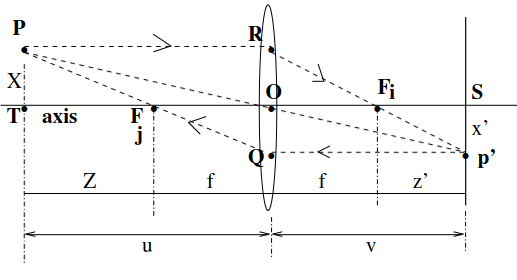
\includegraphics[width=0.5\textwidth]{Figures/ThinLenses.png}
\end{figure}
\\If we move the image plane, point $p'$ is out of focus $\Rightarrow$ $v$ changes $\Rightarrow$ $v'$.
If $P$ is moved $u$ changes $\Rightarrow$ $u'$.
The result is that the image is blurred on the image plane (instead of a point I see a circle, the rays of light don't converge).
\\\textit{NB: If the object is too far you can try to set the focal length but it won't work.}
\begin{figure}[h]
    \centering
    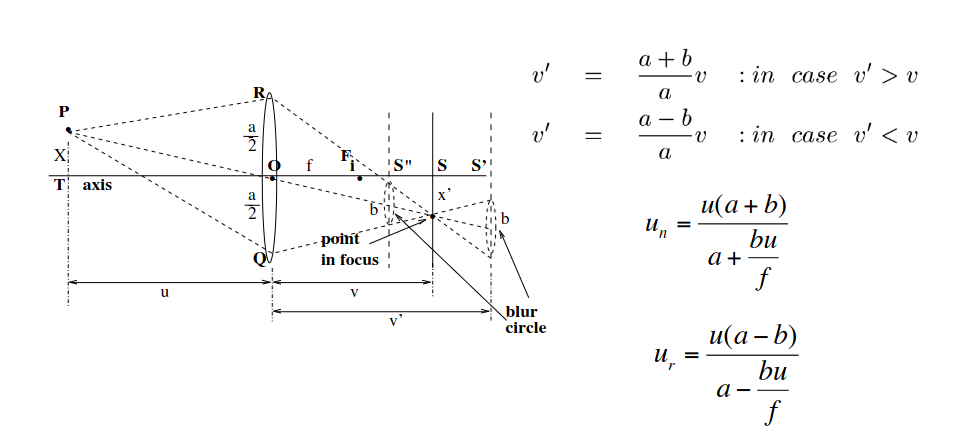
\includegraphics[width=1\textwidth]{Figures/Focus.png}
\end{figure}
\\We want to configure the camera in order to have the quantity $b$ as small as possible.
\\Notice that:
\begin{itemize}
    \item In general $u > f = u_n < u$;
    \item If $f$ becomes smaller, $u_n$ is closer to the camera;
    \item If $f$ becomes smaller, $u_r$ is farther to the camera;
    \item $u_r > u$;
    \item If $u -> \infty$ rays are parallel and converge to the camera center;
    \item The difference between the far and near planes limiting b is called \textit{depth of field}. 
\end{itemize}
\textbf{Autofocus}
\\Is the capability of focusing a specific portion of the image, it can be active, passive or a combination of both.
\\\textbf{Active:}  
\\The camera emits a signal and measures the time it takes to return. The time is used to compute the distance of the object from the camera.
It is mainly used for point-and-shoot cameras. The issues are related to obstacles and glossy and bright surfaces.
\\\textbf{Passive:}
\\The camera uses the contrast of the image to focus. It is mainly used for professional cameras. 
It is more expensive SLR (single-lens reflex) cameras, it uses the phase detection method.
Distance computed using image analysis: take a strip of pixels and analyze the distribution, then if values are too similar the object is out of focus, if contrast is high the object is on focus.
The problems are related to flat surfaces, to low contrast and low light.
Good cameras compute the metric on the vertical and horizontal axes.
